\begin{figure}[h]
  \centering

  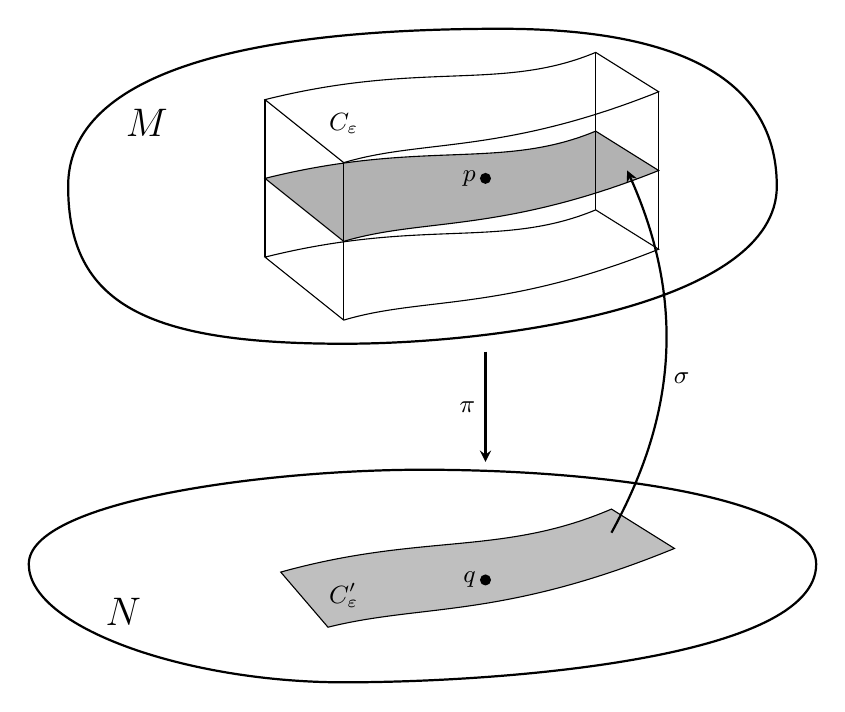
\begin{tikzpicture}[>=stealth, font=\small]

    % --- Manifold N (Bottom) - Flat and elongated ---
    \draw[thick] (-5,0) .. controls (-5,0.8) and (-2,1.2) .. (0,1.2)
    .. controls (2.5,1.2) and (5,0.8) .. (5,0)
    .. controls (5,-1.2) and (1,-1.5) .. (-1,-1.5)
    .. controls (-3,-1.5) and (-5,-0.8) .. (-5,0);
    \node at (-3.8, -0.6) {\Large $N$};

    % Region C'_epsilon in N (The domain)
    \filldraw[fill=gray!50, draw=black] (-1.2, -0.8) .. controls (0, -0.5) and (1, -0.7) .. (3.2, 0.2)
    -- (2.4, 0.7) .. controls (1, 0.1) and (0, 0.4) .. (-1.8, -0.1) -- cycle;

    % \node at (-1,1.5) {$C_\varepsilon$};
    % \fill (0.8, 0.8) circle (2pt) node[left] {$p$};
    \node at (-1,-0.4) {$C'_\varepsilon$};
    \fill (0.8,-0.2) circle (2pt) node[left] {$q$};

    % --- Manifold M (Top) - More "blob-like" and distinct ---
    \begin{scope}[shift={(0,4.8)}]
      \draw[thick] (-4.5,0) .. controls (-4.5,1.8) and (-1,2) .. (1,2)
      .. controls (3,2) and (4.5,1.5) .. (4.5,0)
      .. controls (4.5,-1.5) and (1,-2) .. (-1,-2)
      .. controls (-3.5,-2) and (-4.5,-1.5) .. (-4.5,0);
      \node at (-3.5, 0.8) {\Large $M$};

      \begin{scope}[shift={(0,-0.7)}]
        % Positioning C_epsilon deeper inside M
        % Base height for the central section is now closer to Y=0 (center of M)
        \coordinate (A1) at (-1, -1); \coordinate (B1) at (3, -0.1);
        \coordinate (C1) at (2.2, 0.4); \coordinate (D1) at (-2, -0.2);

        \coordinate (A2) at (-1, 1); \coordinate (B2) at (3, 1.9);
        \coordinate (C2) at (2.2, 2.4); \coordinate (D2) at (-2, 1.8);

        \coordinate (A3) at (-1, 0); \coordinate (B3) at (3, 0.9);
        \coordinate (C3) at (2.2, 1.4); \coordinate (D3) at (-2, 0.8);

        % Draw the top slice of the "cylinder"
        \draw (A2) .. controls (0, 1.3) and (1, 1.1) .. (B2) -- (C2)
        .. controls (1, 1.9) and (0, 2.3) .. (D2) -- cycle;

        % Draw the middle slice (The Local Section)
        \filldraw[fill=gray!60, draw=black] (A3) .. controls (0, 0.3) and (1, 0.1) .. (B3) -- (C3)
        .. controls (1, 0.9) and (0, 1.3) .. (D3) -- cycle;

        % Draw the bottom slice
        \draw (A1) .. controls (0, -0.7) and (1, -0.9) .. (B1) -- (C1)
        .. controls (1, -0.1) and (0, 0.3) .. (D1) -- cycle;

        % Draw the vertical edges
        \draw (A1) -- (A2) (B1) -- (B2) (C1) -- (C2) (D1) -- (D2);

        \node at (-1,1.5) {$C_\varepsilon$};
        \fill (0.8, 0.8) circle (2pt) node[left] {$p$};
      \end{scope}
    \end{scope}

    % --- Maps ---

    % Projection pi (pointed straight down)
    \draw[->, thick] (0.8, 2.7) -- (0.8, 1.3) node[midway, left] {$\pi$};

    % Section sigma (curved upward)
    \draw[->, thick] (2.4, 0.4) .. controls (3, 1.5) and (3.5, 3) .. (2.6, 5)
    node[midway, right] {$\sigma$};

  \end{tikzpicture}

  \caption{Local section of a submersion}
  \label{fig:local_section_of_submersion}
\end{figure}
